% Header: Here are all packages used and some additional definitions
%%%%%%%%%%%%%%%%%%%%%%%%%%%%%%%%%%%%%%%%%%%%%%%%%%%%%%%%%%%%%%%%%%%

\documentclass[11pt,a4paper]{scrartcl}
\usepackage[margin=2.5cm]{geometry}
\usepackage[onehalfspacing]{setspace}
\usepackage{graphicx} % zum Einbinden von Graphiken
\usepackage[breaklinks=true,colorlinks=true,linkcolor=blue,urlcolor=blue,citecolor=blue]{hyperref} % f. Referenzen
\usepackage{amsmath,amsthm,amssymb} % Mathematik Umgebung 
\usepackage{icomma} % Intelligentes Komma, das den richtigen Abstand zwischen Dezimalzahlen als auch in Formeln wählt.
\usepackage[ngerman]{babel} % Deutsche Bezeichnungen bei Inhaltsangabe etc
\usepackage[T1]{fontenc}    % andere Schriftsatzkodierung für richtige Silbentrennung bei Umlauten
\usepackage[locale = DE,space-before-unit=true,per-mode = symbol]{siunitx} % Bessere Einheiten
\usepackage{booktabs,multirow} % Pakete zur Erstellung von Tabellen
\usepackage{placeins} % Definiert den Befehl “\FloatBarrier”, der die Ausgabe der davor eingebundenen Bilder erzwingt, befor der Text weiter geht. (Mit vorsicht zu verwenden)
\usepackage[natbib,abbreviate=true,doi=false,style=numeric-comp,giveninits=true,sorting=none]{biblatex} % Modernes Paket zur Erzeugung von Bibliografien (benötigt biber!)
\usepackage{csquotes} % Fortgeschrittene Funktionen für Zitate, für die deutsche Form der Anführungszeichen bei Referenzen
\addbibresource{MyBibliography.bib} % Ort der .bib Datei, die die Datenbank für Literatur/Referenzen enthält.

\graphicspath{{Bilder/}}

\DeclareSIUnit{\dBm}{dBm}
\DeclareSIUnit[per-mode=reciprocal]\WN{\per\centi\meter}

%%%%%%%%%%%%%%%%%%%%%%%%%%%%%%%%%%%%%%%%%%%%%%%%%%%%%%%%%%%%%%%%%%%
\begin{document}
%
\titlehead{
\includegraphics[width=5cm]{logo.jpg}}
\title{Titel des Berichts}
\author{Student Eins\thanks{\href{mailto:Email.Student1@uibk.ac.at}{Email.Student1@uibk.ac.at}}, Student Zwei\thanks{\href{mailto:Email.Student2@uibk.ac.at}{Email.Student2@uibk.ac.at}}}
\date{\today}
\maketitle
\vfill
\section*{\abstractname}
\textit{Wenn man nur 2 Minuten hätte um einem Kollegen/einer Kollegin die Arbeit zu erklären, was soll er/sie davon wissen?}
\thispagestyle{empty}
%
%
\tableofcontents
\thispagestyle{empty}
\cleardoublepage
\pagenumbering{arabic} 
\newpage
%
%
\section{Einleitung}
\label{sec:Einleitung}
%
\textit{Worum geht es in dem Versuch? Was ist die Hauptfrage und warum ist sie interessant?}\\
Im Anhang~\ref{sec:Latex} finden Sie einige Informationen, die hilfreich für den Einstieg in \LaTeX{} sein könnten.
%
\section{Grundlagen und Theorie}
\label{sec:Grundlagen}
%
\textit{Was sind die wichtigen physikalischen Grundlagen?}\\
Tabelle \ref{tab:exapltab} zeigt ein typisches Beispiel für eine Tabelle in einer Auswertung.
\begin{table}[htbp]
\centering
\caption{\label{tab:exapltab}Dies hier ist eine typische Tabelle. Die Werte haben, wenn nicht anders angegeben, eine Unsicherheit von \SI{0,4}{\nano\meter}. Da die lateralen Dimensionen von Teilchen D (in einer Dimension) stark vom Mittelwert abweichen, wurde der Mittelwert zusätzlich ohne dieses Teilchen berechnet.}
\begin{tabular}{cccccc}
\toprule
\multicolumn{1}{c}{Teilchen}	& \multicolumn{1}{c}{Länge / \si{\nano\meter}}		& \multicolumn{1}{c}{Breite / \si{\nano\meter}}	& \multicolumn{1}{c}{Höhe / \si{\nano\meter}} \\
\midrule
\multirow{1}{*}{A} & $34,5$	& $25,6$		& $4,6$		  \\
\multirow{1}{*}{B} & $34,4$	& $28,0$		& $4,0$		  \\
\multirow{1}{*}{C} & $31,9$	& $27,4$		& $4,6$		  \\
\multirow{1}{*}{D} & $49,1$	& $34,0$		& $4,6$		 \\
\multirow{1}{*}{E} & $35,2$	& $26,1$		& $4,9$		 \\
\multirow{1}{*}{F} & $27,2$	& $23,6$		& $4,3$		\\  
\multirow{1}{*}{G} & $27,2$	& $23,6$		& $4,3$		  \\
\midrule
\multirow{1}{*}{Mittelwert:} & $35\pm6$	& $28\pm3$		& $4,7\pm0,6$	\\	  
\multirow{1}{*}{Mittelwert} & \multirow{2}{*}{$33\pm3$}	& \multirow{2}{*}{$27\pm2$}		& \multirow{2}{*}{}	\\	  
\multirow{1}{*}{ohne Teil.\ D:} & 	& & \\	  
\bottomrule
\end{tabular}
\end{table}
%
\section{Experiment und Aufbau}
\label{sec:ExpAufb}
%
\textit{Was würde jemand brauchen, um den Versuch nachzuvollziehen und zu wiederholen?}\\
Als Beispiel für eine Gleichung ist hier die Formel für das Verhalten eines verkippbaren Interferenz-Filters angegeben. Dabei verschiebt sich die Wellenlänge $\lambda\left(\Phi\right)$ der Filterkante bei größeren Winkeln $\Phi$, unabhängig von der Kipp"=Richtung, zu kürzeren Wellenlängen~\cite{TiltFilter}:
\begin{equation}
\lambda\left(\Phi\right)=\lambda\left(0\right)\sqrt{1-\frac{\sin^2\Phi}{n_\text{eff}^2}}\;.
\label{eq:TiltWel}
\end{equation}
$n_\text{eff}$ ist der effektive Brechungsindex.
%
\section{Ergebnisse}
\label{sec:Ergebnisse}
%
\textit{Was ist(sind) die gemessene Antwort(en) auf die Hauptfrage(n)?}\\
Abbildung \ref{fig:examplfig} zeigt ein Beispiel für eine Abbildung in Haupttext.
\begin{figure}[htb!]
 \centering
 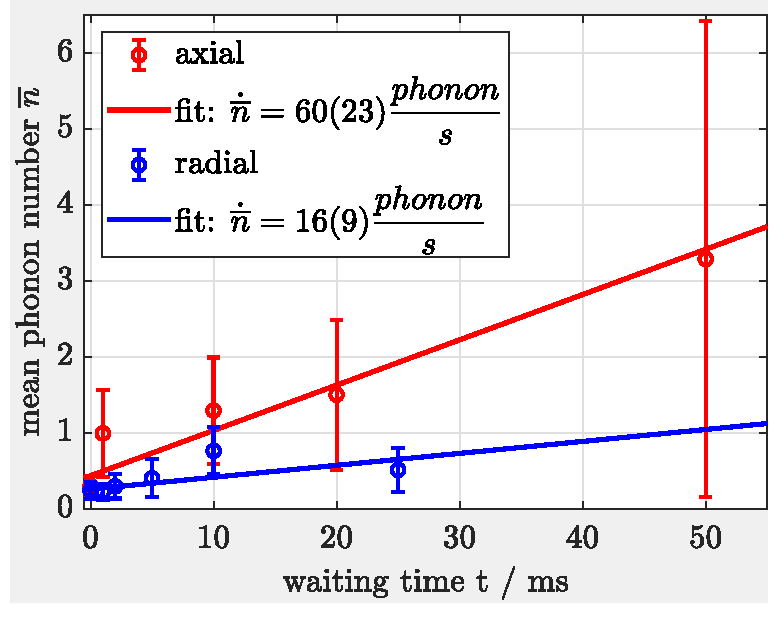
\includegraphics[width=0.65\textwidth]{good_example_plot}
 \caption{\label{fig:examplfig}Ein typischer Graph in einer Auswertung.
 }
\end{figure}
%
\section{Schlussfolgerungen}
\label{sec:Schlussf}
%
\textit{Was ist die Endantwort und soll ihr vertraut werden?  Wie hätte man den Versuch anders oder besser durchführen können?}\\
Die Referenz~\cite{GP1StromSpannung} soll ein Beispiel sein, wie man ein Praktikums"=Skript zitieren sollte. 
%
\newpage
\appendix
\section{Ein paar Tipps und Tricks für \LaTeX}
\label{sec:Latex}
%
Dieses Dokument soll keine vollständige Anleitung darstellen, wie das Textsatzsystem \LaTeX{}  funktioniert. Hierfür gibt es eine Menge an guten Internetquellen. Wir wollen Ihnen einen kleinen Überblick verschaffen, damit der Einstieg leichter fällt, und eine Vorlage geben, mit denen Sie mit möglichst wenig Aufwand Ihren Bericht schreiben können. Viele Befehle werden hier nicht näher erklärt, aber deren Gebrauch sollte sich aus dem Quelltext ergeben. Grundsätzlich benötigen Sie zunächst eine TeX-Distribution, wie z.B.\ MiKTeX für Windows, das kostenlos aus dem Internet heruntergeladen werden kann. Diese übersetzen den Quelltext in eine PDF"=Datei. Ein zusätzlicher Texteditor zum Erstellen des Quelltextes, z.B.\ TeXnicCenter, ist sehr hilfreich. Dieser enthält viele Werkzeuge und Hilfsmittel, z.B.\ einen Überblick über die Gliederung oder Autovervollständigung und vieles mehr. Der Quelltext kann auch in mehrere Dateien aufgeteilt werden und mit dem Befehl \verb+\include{}+ oder \verb"\input{}" werden die Dateien eingefügt, so wie es hier mit dem Anhang gemacht wird. Die meisten Editoren enthalten auch einen Dokumentenbetrachter für die fertige PDF. Manche benötigen hierfür allerdings ein weiteres Programm. Hier kann z.B.\ Adobe Acrobat Reader oder Sumatra, das für die Verwendung mit \LaTeX{} optimiert ist, verwendet werden. Es gibt hier eine Vielzahl verschiedener Lösungen; viele Studenten benutzen heutzutage die Online"=\LaTeX"=Umgebung Overleaf, welche keine lokale Installation der \LaTeX"=Distribution benötigt und es ermöglicht als Team an einem Dokument gleichzeitig zu arbeiten.
%
\subsection{Header, Dokumentenklasse und Gliederung}
\label{subsec:DokHeadGli}
Im Header, also bevor das Dokument mit \verb+\begin{document}+ begonnen wird, wird zunächst die Dokumentenklasse \verb+scrartcl+ festgelegt. Es gibt hier einige vordefinierte Klassen, die für die jeweilige Art des Dokuments optimiert sind. Darunter werden mit dem Befehl \verb+\usepackage{}+ die benötigten Pakete geladen. Diese müssen natürlich installiert sein, was viele \LaTeX"=Distributionen automatisch machen. Zusätzlich können den Paketen in den eckigen Klammern ggf.\ diverse Optionen übergeben werden. Der Header ist auch der optimale Ort, um weitere Definitionen zu machen.\\
Dieses Dokument verwendet das moderne Paket BibLaTeX zur Erzeugung des Literaturverzeichnis, eine komplette Neuimplementierung des bisher meistens verwendeten BibTeX. \LaTeX{} erzeugt das Literaturverzeichnis nicht direkt selber, sondern benutzt dafür ein "`externes Programm"'. Um ein Dokument mit seinem Haupttext und dem Literaturverzeichnis vollständig zu erzeugen, muss zuerst der latex"=Compiler (z.B.\ pdflatex) das Hauptdokument sowie eine *.bbl Datei erzeugen. Diese Datei enthält die Informationen über die zitierten Referenzen. Anschließend erzeugt das externe Programm das Literaturverzeichnis. Diese beiden Schritte werden von den meisten \LaTeX"=Editoren automatisch ausgeführt. Anschließend benötigt es eine erneute Ausführung des latex"=Compilers, damit das aktualisierte Literaturverzeichnis in das Hauptdokument (die PDF) eingefügt wird. Das ist der Grund warum, bei der Verwendung von BibTeX oder BibLaTeX der Compilierungsprozess ggf.\ öfters ausgeführt werden muss. Beachten Sie, dass BibLaTeX das externe Programm biber benötigt. Falls ihr Editor mit BibTeX konfiguriert ist, finden Sie z.B.\ in der Referenz~\cite{bibtextobiber,biblatex} eine Anleitung für die Umstellung des externen Programms von bibtex zu biber bzw.\ weitere Informationen.\\
Die Kurzfassung wurde mit dem Befehl \verb"\section*{\abstractname}" begonnen. Der Befehl \verb"\section{}" erzeugt ein neues Kapitel, wobei die Kapitelüberschrift in den geschweiften Klammern steht. Unterkapitel werden mit \verb"\subsection{}" usw.\ begonnen, wobei die Gliederung in manchen Klassen mit \verb"\chapter{}" beginnt, dann \verb"\section{}", usw.  Der \verb"*" bewirkt, dass dieses Kapitel nicht in die Inhaltsangabe aufgenommen wird und auch nicht nummeriert wird.\\
Sehr viele Dinge sind in den verschiedenen \LaTeX"~Klassen, hier \textit{scrartcl} bereits vordefiniert. Da die Dokumentensprache in der Option (in den eckigen Klammern) des Sprachpakets \textit{babel} mithilfe des Befehls \verb"\usepackage[ngerman]{babel}" auf Deutsch gesetzt wurde, übersetzt Latex z.B.\ den Befehl \verb"\abstractname" mit \abstractname.
%
\subsection{Befehle, Leerzeichen und Kommentare}
\label{subsec:TextBefehle}
Vor Befehlen steht, außer es sind Zeichen die im normalen Text nicht vorkommen, immer ein Backslash ($\backslash$). Die häufigsten Befehle im Fließtext werden Leerzeichen ($\backslash$) und Zeilenumbrüche sein ($\backslash\backslash$ oder \verb"\newline"). Hier kann es hilfreich sein zu wissen, dass je nach Einstellungen, \LaTeX{} nach einem Punkt einen größeren Abstand einfügt. Dies muss bei einem Punkt nach einer Abkürzung unterdrückt werden, wie z.B.\ hier. Der Abstand bei einem Zeilenumbruch kann z.B.\ mit \verb"\\[5ex]" vergrößert werden, wobei hier \verb"ex" eine der vielen Längeneinheiten in \LaTeX{} ist.\\
Nachdem das Dokument auf Deutsch eingestellt ist, wird \LaTeX{} automatisch die Silbentrennung nach Regeln der deutschen Rechtschreibung bei Zeilenumbrüchen durchführen. Dies kann oft auch zu ungewollten Ergebnissen führen, die mit Sonderzeichen, wie z.B.\ \verb+"=+ behoben werden können \cite{Silbentrennung}.
Je nach Einstellung werden Zeilenumbrüche im Quelltext ignoriert.\\
Alles was im Quelltext nach dem \%"~Zeichen steht wird vom Interpreter ignoriert. Dies erlaubt uns den Quelltext mit hilfreichen Kommentaren zu versehen. % Vielleicht sollte ich hier noch etwas über Fahrräder schreiben.
% Das "~ Zeichen musste ich jetzt selber nachschauen.
Mit dem Befehl \verb"\footnote{}" werden Fußnoten\footnote{Man sollte es aber nicht mit Fußnoten übertreiben.} erstellt.
\subsection{Mathematik}
\label{subsec:Mathematik}
Gleichungen können direkt in den Text $\sum_{i=1}^{k+1}i$ geschrieben werden oder in einer \verb"equation" Umgebung abgesetzt werden:
\begin{equation}
E=mc^2 \label{eq:einstein}
\end{equation}
In den Paketen \textit{amsmath}, \textit{amsthm} und \textit{amssymb} sind bereits viele Symbole und typische Ausdrücke definiert:
\begin{equation}
\label{eq:abg}
\lim_{x \to 0} \frac{\ln \sin \pi x}{\ln \sin x} = 
     \lim_{x \to 0} \frac{\pi \frac{\cos \pi x}{\sin \pi x} }{ \frac{\cos x}{\sin x} } =
     \lim_{x \to 0} \frac{\pi \tan x}{\tan \pi x} = \quad \ldots \quad = 1 \, .
\end{equation}
\begin{equation}
\label{eq:matrix}
\mathcal{A} = \left( \begin{array}{ccc} 6 & 0 & 0 \\ 0 & 5 & 0 \\ 0 & 1 & 2 \end{array} \right)\, , \quad
\mathcal{B} = \left( \begin{array}{ccc} 1 & 2 & 3 \\ 2 & 1 & 0 \\ 4 & 3 & 0 \end{array} \right)\, \Rightarrow
\mathcal{A} \cdot \mathcal{B} = \left( \begin{array}{ccc} 6 & 12 & 18 \\ 10 & 5 & 0 \\ 10 & 7 & 0 \end{array} \right)
\end{equation}
In der Umgebung \verb"align" können mehrere Zeilen mithilfe des \verb"&" Zeichen aufeinander ausgerichtet werden
\begin{align}
\alpha + \beta &=\gamma^2 \\
\alpha^2 + 2\gamma + \cos\theta &= \delta. \mathrm{a}\label{eq:erstesBsp} 
\end{align}

\begin{align}
\alpha + \beta &=\gamma^2 \\
\alpha^2 + 2\gamma + \cos\theta &= \delta.\label{eq:zweitesBsp} 
\end{align}

\subsection{Einheiten und Dezimalzahlen}
\label{sec:Einheiten}
 In der Mathematik"=Umgebung werden Buchstaben automatisch kursiv geschrieben, Einheiten dürfen aber nicht kursiv geschrieben werden. Zusätzlich muss zwischen Zahlenwert und Einheit ein kleiner Abstand eingefügt werden. Mithilfe des \textit{siunitx} Pakets ist es sehr einfach Einheiten im Fließtext und in den Mathematik"=Umgebungen mit einer sauberen Formatierung zu setzen. Man kann mithilfe des Befehls \verb"\si{}" die Einheit alleine ausgeben \verb"\si{\meter\per\second\squared}" wird zu \si{\meter\per\second\squared}. Alternativ kann man auch den Zahlenwert mithilfe des \verb"\SI{}{}" Befehls übergeben. Dies wird empfohlen, da hier unter Anderem der notwendige Abstand zwischen Zahl und Einheit automatisch erzeugt wird, sowie automatisch das deutsche Dezimaltrennzeichen , verwendet wird. Hier ein paar Beispiele:
\begin{align*} \label{eq:einhbsp}
r&=\SI{430}{\micro\meter}\; , \\
A&=\SI{3,53}{\centi\meter\squared}\; , \\
A&=\SI{3.53}{\centi\meter\squared}\; , \\
\rho&=\SI{0,7914}{\gram\per\cubic\centi\meter} \; , \\
\eta&=\SI{5,95e-4}{\kilo\gram\per\meter\per\second} = \SI{5,95e-4}{\pascal\second} \; .
\end{align*}
Das \textit{siunitx} Paket kann sich auch um die Formatierung der Angabe der Unsicherheit kümmern:
\begin{align*}
\theta& =\SI[separate-uncertainty=false]{5,95(14)e-4}{\pascal\second}\; ,\\
\theta& =\SI[separate-uncertainty=false]{5,95\pm0.14 e-4}{\pascal\second}\; ,\\
\theta& =\SI[separate-uncertainty=true]{5,95(14)e-4}{\pascal\second}\; ,\\
\theta& =\SI[separate-uncertainty=true]{5,95\pm0.14 e-4}{\pascal\second}\; .
\end{align*}
Man kann auch selber Einheiten definieren mit dem Befehl \verb"\DeclareSIUnit{}{}" im Header, z.B.\  \verb"\DeclareSIUnit{\dBm}{dBm}": \verb"\si{\dBm}" wird zu \si{\dBm}.\\
\LaTeX{} macht typischerweise in der Mathematik"=Umgebung einen keinen Abstand nach einem Komma. Dies sollte bei Dezimalzahlen nicht der Fall sein. Eine Lösung dafür ist eine geschweifte Klammer um das Komma zu machen, z.B.\ $1{,}5$. Alternativ kann man, wie in diesem Dokument, das Paket \textit{icomma} verwenden, wodurch der Abstand in Dezimalzahlen automatisch weggelassen wird.
\subsection{Tabellen und Listen}
\label{subsec:Tabellen}

Tabelle \ref{tab:TempabhVerteilung} zeigt ein Beispiel wie man Tabellen einfügen kann. Das Paket \textit{booktabs} erlaubt es sehr übersichtliche Tabelle zu erstellen. Das Paket \textit{multirow} kann sehr hilfreich sein, wenn Text über mehrere Zeilen geschrieben werden soll. Es gibt auch Tools, um Tabellen von Excel \& Co. nach Latex zu exportieren, was sehr viel Zeit sparen kann, siehe "`excel2latex"'~\cite{extolat}.
\begin{table}[htbp]
\centering
\caption{\label{tab:TempabhVerteilung}Mittelwert $\nu_0$ und Halbwertsbreite FWHM der Verteilung der ZPLs in Abhängigkeit der Temperatur. Die Parameter wurden jeweils mithilfe eines Gauß"=Fits an die Verteilung bestimmt und durch direkte Berechnung des Mittelwerts bzw.\ der Umrechnung der Standardabweichung in die FWHM der Normalverteilung.}
\begin{tabular}{ccccccc}
\toprule
\multicolumn{2}{c}{Temperatur / \si{\kelvin}}	& \multicolumn{1}{c}{alle}		& 2,0(3)		& 6,5(5)		& 9,0(3) & 12,0(5) \\
\midrule
\multirow{2}{*}{Gauß"=Fit:} & \multicolumn{1}{c}{$\nu_0/\si{\WN}$}	& 1882(2)		& 1882(5)		& 1883(2) & 1884(1,4) & 1887(3) \\
														&	\multicolumn{1}{c}{FWHM$/\si{\WN}$}		& 22,3(1,5)			& 19,9(1,2)			& 31(2) 	& 36(1) 	& 40(2) \\
\midrule
\multirow{2}{*}{Statistik:} & \multicolumn{1}{c}{$\nu_0/\si{\WN}$}	& 1885(3)		& 1883(8)		& 1884(4) & 1885(3) & 1888(2) \\
														& \multicolumn{1}{c}{FWHM$/\si{\WN}$}		& 32(4)			& 26(2)			& 32(2) 	& 37(5) 	& 36(2) \\
\bottomrule
\end{tabular}
\end{table}\\
Berichte sollten immer im Blocksatz geschrieben werden. Das gilt auch für Aufzählungen, wie z.B.\ für die Berichte für die Versuche "`Kalibrierung und das hookesche Gesetz"', "`Einfacher harmonischer Oszillator"', "`Schallgeschwindigkeit"' und "`Magnetfelder"'. Falls unbedingt notwendig kann man mit der \verb"itemize" Umgebung mehrere Punkte in einer Liste anführen:
\begin{itemize}
    \item Erster Punkt,
    \item Zweiter Punkt,
    \item Dritter Punkt.
\end{itemize}


\subsection{Label und Referenzen}
\label{subsec:labelref}
Man kann Kapitel, Tabellen, Abbildungen, Gleichungen usw.\ mit \verb"\label{}" mit einem Label versehen. Anschließend kann man mithilfe des Befehls \verb"\ref{}" auf ein Kapitel~\ref{subsec:TextBefehle}, eine Tabelle~\ref{tab:TempabhVerteilung}, ein Bild~\ref{fig:figureone} oder eine Gleichung~\ref{eq:zweitesBsp} verweisen. Dabei muss man im Text immer explizit anführen, ob es sich um ein Kapitel, eine Gleichung, etc.\ handelt. % Der Zusatz tab:, fig:, eq:, etc. im Label hat keine explizite Bedeutung für LaTeX, sondern ist nur hilfreich zur Übersichtlichkeit.
%
\subsection{Zitieren von Referenzen}
\label{subsec:ZitRef}
In der Datei "`MyBibliography.bib"' gibt es eine Liste an Literaturquellen, auf die u.A.\ mit dem Befehl \verb"\cite{}" referenziert werden kann. Es gibt eine Reihe verschiedenen Literaturtypen, wie z.B.\ \textit{article}, \textit{book} oder \textit{misc}, die wiederum verschiedene Felder, wie z.B.\ \textit{title}, \textit{author} oder \textit{url} anbieten~\cite{biblatexManual}. Je nach Literaturtyp wird der Eintrag auch unterschiedlich im Literaturverzeichnis formatiert. Gelegentlich will man nicht, dass z.B.\ Autorennamen abgekürzt werden oder der Anfangsbuchstaben im Title klein geschrieben werden. Dies kann man mit geschweiften Klammern erreichen. Umlaute im Literaturverzeichnis führen oft zu Problemen. Dies kann behoben werden, indem man anstatt der Umlaute direkt, z.B.\ \verb+ä+, \verb+ü+, \verb+ö+, etc.,\ die Sonderzeichen \verb+\"a+, \verb+\"u+, \verb+\"o+, etc.\ verwendet.\\
Mehr Information \"uber Physik ist in den Referenzen \cite{Demtroeder3,PhysRev.47.777} zu finden. Ref.~\cite{Internetquelle1} und Ref.~\cite{Internetquelle2} sind Beispiele von Internet"=Quellen.
%
\subsection{Abbildungen}
\label{subsec:Abb}
Abbildung~\ref{fig:figureone} zeigt wie eine Abbildung in der Gleitumgebung \verb"figure" eingefügt werden kann. Die Optionen \verb"[htb!]" definieren wie die Abbildung platziert werden soll.
\begin{figure}[htb!]
 \centering
 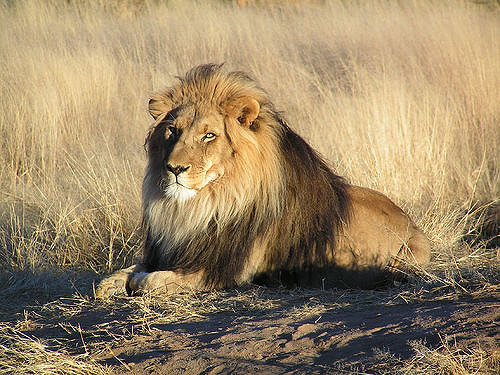
\includegraphics[width=10cm]{lion.jpg}
 \caption{\label{fig:figureone}  Ein Bild von einem Löwen. Bild übernommen von Referenz \cite{Internetbildquelle}.}
\end{figure}\\
%
Abbildung \ref{fig:vieleBilder} zeigt ein Beispiel, wie thematisch zusammengehörende Unterabbildungen in eine Abbildung eingefügt werden können. Abbildung \ref{fig:vieleBilder} unten zeigt ein Histogramm. 
%
\begin{figure}[h!tb]
\centering
  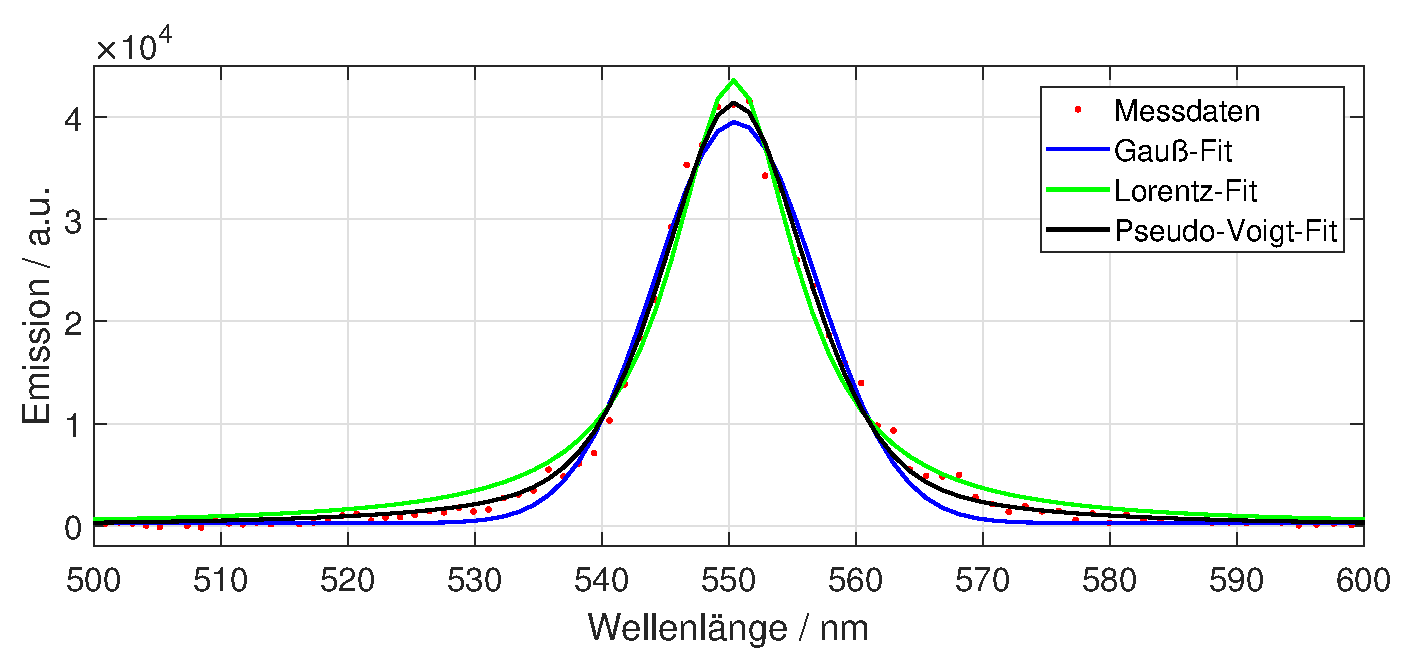
\includegraphics[width=0.9\linewidth]{SMEmi_170922_FitBeispiel}
\hfill
  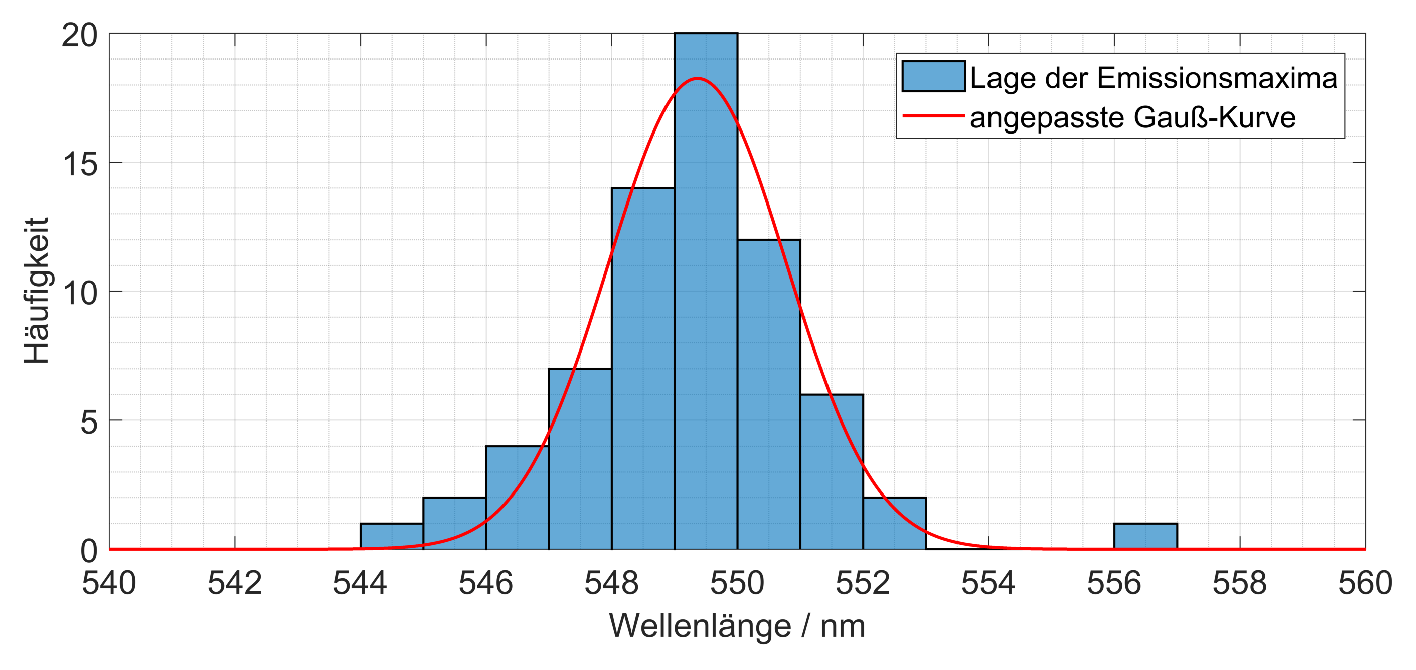
\includegraphics[width=.9\linewidth]{SMEmi_170922_Histogram}
\caption{Emissions"=Spektroskopie an einzelnen CdSe"=Nanoplatelets bei Raumtemperatur. Analyse der Messungen vom 22.09.17. Für weitere Informationen über die Messparameter siehe Text. Oben: Beispiel für die Anpassung der verschiedenen Modelle an eines der Emissions"=Spektren. Das gemessene Emissions"=Profil wird am besten durch das Pseudo"=Voigt"=Profil beschrieben. Im Mittel weisen die Emissions"=Spektren eine Halbwertsbreite von $\SI{14}{\nano\meter}$ auf. Unten: Histogramm der Verteilung der durch die Fits bestimmte spektrale Lage der Emissions"=Spektren. Die an die Verteilung angepasste Gauß"=Kurve lieferte eine mittlere Lage von $\SI{549,2}{\nano\meter}$ und eine Halbwertsbreite der Verteilung von $\SI{3,3}{\nano\meter}$.}
\label{fig:vieleBilder}
\end{figure}
\newline
\FloatBarrier
%
\subsection{Zusammenfassung}
\label{subsec:ZusammenLatex}
%
Wir hoffen, dass Ihnen mit diesem kleinen Dokument der Einstieg in \LaTeX{} etwas leichter fällt. Abschießend bleibt zu sagen, dass für nahezu jedes Problem, das auftaucht, eine Lösung gefunden werden kann, man muss sie nur finden. % Der Anhang ist in einer externen Datei "Anhang.tex" und wird hier in das Dokument eingefügt.

\printbibliography[]
\vfill
\section*{Erklärung}

Hiermit versichern wir, dass der vorliegende Bericht selbständig verfasst wurde und alle notwendigen Quellen und Referenzen angegeben sind.

\begin{tabular}{@{}p{2.5in}p{2.5in}@{}}
 \\[5\bigskipamount]
  \dotfill & \dotfill \\
  Student 1 & Date \\[5\bigskipamount]
  \dotfill & \dotfill \\
 Student 2 & Date \\
  \centering
  
\end{tabular}

\end{document}
